This is the week 1 of the course Probabilistic Graphical Models (pgm) by Prof. Daphne Koller hosted on Coursera. The week 1 covers quite a lot of notions from distribution to Bayesian Network.

\section{Distribution}
A probability distribution function (aka PDF, probability density function, probability function, or density) is a function that indicates the probability that a given random variable will take on a particular value. If a random variable is discrete (i.e. the value of the random variable is contained in a countable set of values), then the probability density function, $f(x)$ of a random variable $X$ is: $f(x) = \mathbb{P}(X = x)$.\\

The multivariate form of a probability distribution function is the probability that a list of random variables will take on a list of values. If the random variables are discrete, the \textbf{joint probability density function}, $f(x_1, x_2, …, x_n)$ for random variables $X_1, X_2, ..., X_n$ is defined by: 
\begin{align}
f(x_1, x_2, \ldots, x_n) = P(X_1=x_1, X_2=x_2, \ldots, X_n=x_n)
\end{align}
\myaligns{Joint Distribution}

\section{Factors}
A factor is a function or a table or a mapping from every assignment of arguments to a real value. We define below factor $\Phi(X_1, \ldots, X_k)$ where $(X_1, \ldots, X_k)$ which is the scope (a set of random variables).
\begin{align}
\Phi: Val(X_1, \ldots, X_k) \rightarrow \mathbb{R}
\end{align}
\myaligns{Factor Definition}

\subsection{Examples of Factor}
Hence, according to the definition above, a joint distribution is a factor. Figure \ref{w1JointDistri} illustrates a joint distribution $\mathbb{P}(I,D,G)$ where $I$, $D$, $G$ represents intelligence of a student $(0, 1)$, difficulty of a course $(0,1)$, and the final grade $(A,B,C)$ that student got from that course respectively.
\begin{figure}[!ht]
\centering
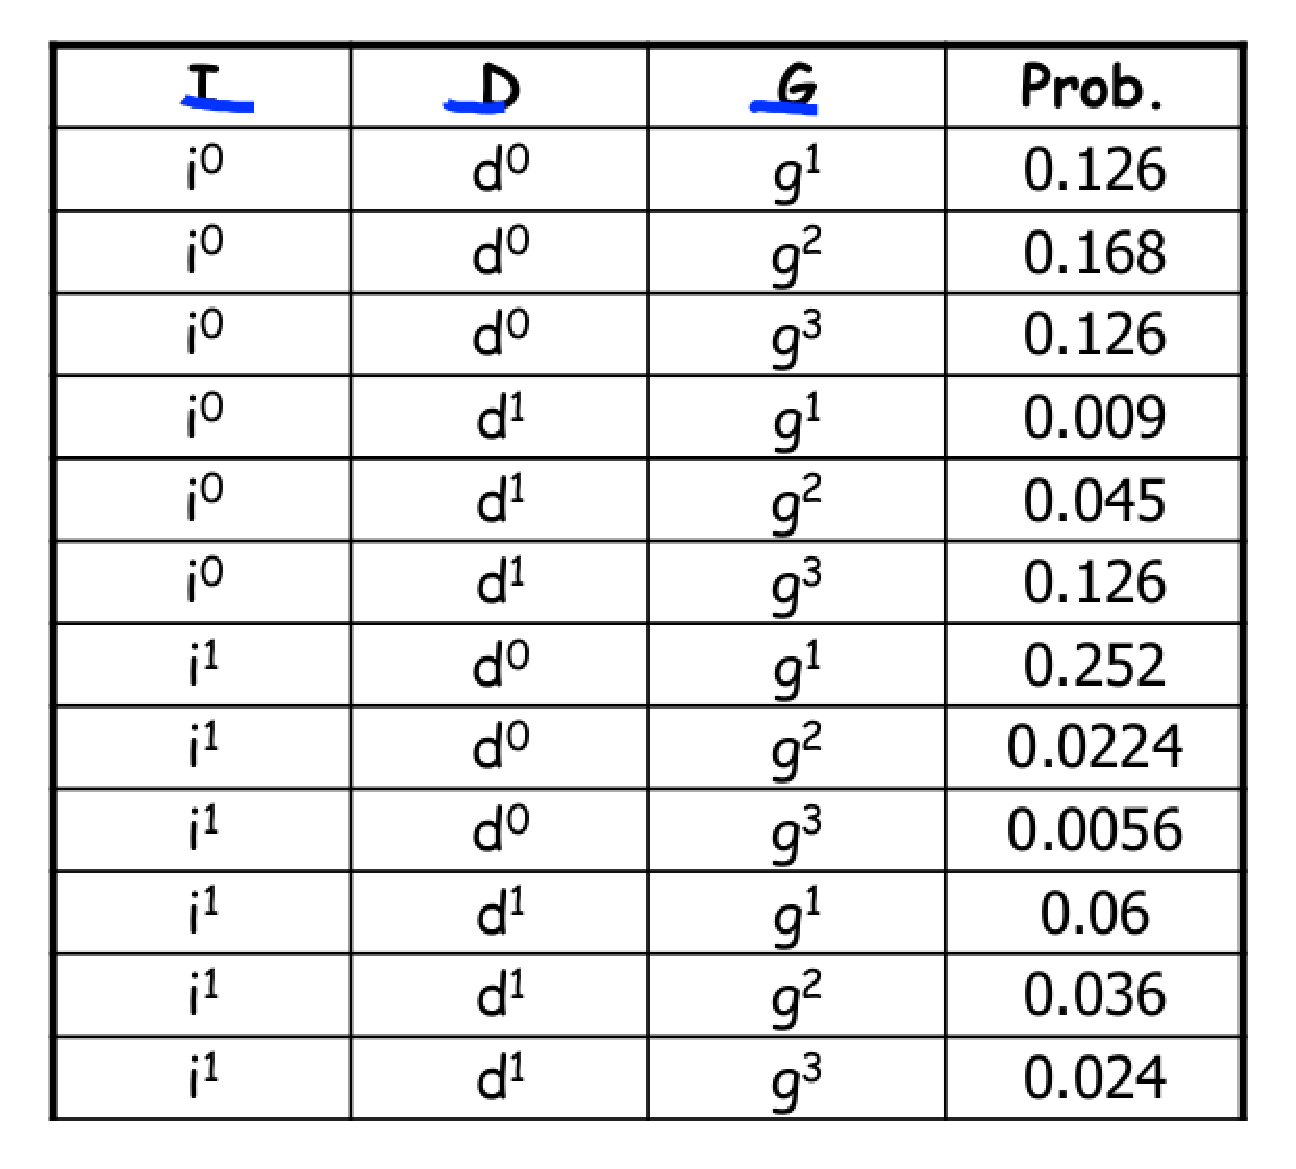
\includegraphics[scale = 0.6]{w1JointDistri}
\caption{bla bla}
\label{w1JointDistri}
\end{figure}

\section{Operations on Factors}